\documentclass[tikz,border=4pt]{standalone}
\usepackage{libertine}
\usepackage{amsmath,amssymb}
\usepackage{pgfplots}
\usetikzlibrary{arrows.meta}
\pgfplotsset{compat=1.18}
\begin{document}
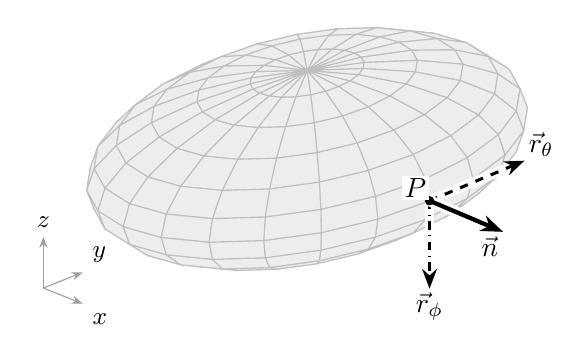
\begin{tikzpicture}
\begin{axis}[
  view={45}{25},
  x={(0.7778cm,-0.3287cm)},y={(0.7778cm,0.3287cm)},z={(0cm,0.9969cm)},
  xmin=-2.4,xmax=3.25,ymin=-3.4,ymax=3.5,zmin=-1.5,zmax=1.4,
  axis lines=none,ticks=none,clip=false,
  axis line style={gray!65,thin,-{Stealth[length=1.5mm]}},
  every axis label/.style={font=\small},
  z buffer=sort]
\addplot3[surf,shader=flat,draw=gray!50,fill=gray!14,
  samples=25,samples y=13,domain=0:360,y domain=0:180]
  ({2*sin(y)*cos(x)},{3*sin(y)*sin(x)},{cos(y)});
% P=(2,0,0); all arrows are positive multiples of the named vectors.
\draw[white,line width=3.5pt] (axis cs:2,0,0)--(axis cs:2,1.55,0);
\draw[black,dashed,line width=1.1pt,-{Stealth[length=2.5mm]}]
  (axis cs:2,0,0)--(axis cs:2,1.55,0)
  node[above right,fill=white,inner sep=1pt] {$\vec r_\theta$};
\draw[white,line width=3.5pt] (axis cs:2,0,0)--(axis cs:2,0,-1.12);
\draw[black,dash dot,line width=1.1pt,-{Stealth[length=2.5mm]}]
  (axis cs:2,0,0)--(axis cs:2,0,-1.12)
  node[below,fill=white,inner sep=1pt] {$\vec r_\phi$};
\draw[white,line width=4pt] (axis cs:2,0,0)--(axis cs:3.2,0,0);
\draw[black,line width=1.55pt,-{Stealth[length=2.8mm]}]
  (axis cs:2,0,0)--(axis cs:3.2,0,0)
  node[below left,fill=white,inner sep=1pt] {$\vec n$};
\fill (axis cs:2,0,0) circle (1.7pt)
  node[above left,fill=white,inner sep=1pt] {$P$};
\end{axis}
% Small coordinate triad, separated from the surface and frame arrows.
\begin{scope}[shift={(current bounding box.south west)},x=1cm,y=1cm]
\coordinate (O) at (-.55,.45);
\draw[gray!75,thin,-{Stealth[length=1.4mm]}] (O)--++(.5,-.2) node[below right,text=black,font=\small] {$x$};
\draw[gray!75,thin,-{Stealth[length=1.4mm]}] (O)--++(.5,.2) node[above right,text=black,font=\small] {$y$};
\draw[gray!75,thin,-{Stealth[length=1.4mm]}] (O)--++(0,.65) node[above,text=black,font=\small] {$z$};
\end{scope}
\end{tikzpicture}
\end{document}
